\documentclass[
ngerman,
twoside,
pdfa=false,
ruledheaders=section,%Ebene bis zu der die Überschriften mit Linien abgetrennt werden, vgl. DEMO-TUDaPub
class=report,% Basisdokumentenklasse. Wählt die Korrespondierende KOMA-Script Klasse
thesis={type=sta},% Dokumententyp Thesis, für Dissertationen siehe die Demo-Datei DEMO-TUDaPhd
accentcolor=TUDa-2c,% Auswahl der Akzentfarbe
custommargins=false,% Ränder werden mithilfe von typearea automatisch berechnet
marginpar=false,% Kopfzeile und Fußzeile erstrecken sich nicht über die Randnotizspalte
%BCOR=5mm,%Bindekorrektur, falls notwendig
parskip=half-,%Absatzkennzeichnung durch Abstand vgl. KOMA-Sript
fontsize=11pt,%Basisschriftgröße laut Corporate Design ist mit 9pt häufig zu klein
%	logofile=tuda_logo.pdf, %Falls die Logo Dateien nicht installiert sind
]{tudapub}

%%%%%%%%%%%%%%%%%%%%%%%%%%%%
% Download des TU-Logos
%%%%%%%%%%%%%%%%%%%%%%%%%%%%
% https://download.hrz.tu-darmstadt.de/protected/CE/TUDa_LaTeX/tuda_logo.pdf
% Der Pfad zum Logo kann als "logofile" angegeben werden.

%%%%%%%%%%%%%%%%%%%
% Sprachanpassung & Verbesserte Trennregeln
%%%%%%%%%%%%%%%%%%%
\usepackage[english, main=ngerman]{babel}
\usepackage[autostyle]{csquotes}% Anführungszeichen vereinfacht
\usepackage{microtype}

%%%%%%%%%%%%%%%%%%%
% Literaturverzeichnis
%%%%%%%%%%%%%%%%%%%
\usepackage{biblatex}   % Literaturverzeichnis
\addbibresource{HausarbeitBib.bib}

%%%%%%%%%%%%%%%%%%%
% Paketvorschläge Tabellen
%%%%%%%%%%%%%%%%%%%
%\usepackage{array}     % Basispaket für Tabellenkonfiguration, wird von den folgenden automatisch geladen
\usepackage{tabularx}   % Tabellen, die sich automatisch der Breite anpassen
%\usepackage{longtable} % Mehrseitige Tabellen
%\usepackage{xltabular} % Mehrseitige Tabellen mit anpassarer Breite
\usepackage{booktabs}   % Verbesserte Möglichkeiten für Tabellenlayout über horizontale Linien

%%%%%%%%%%%%%%%%%%%
% Paketvorschläge Mathematik
%%%%%%%%%%%%%%%%%%%
\usepackage{mathtools} % erweiterte Fassung von amsmath
\usepackage{amssymb}   % erweiterter Zeichensatz
\usepackage[decimalsymbol=comma]{siunitx}   % Einheiten
\usepackage{amsmath}


%%%%%%%%%%%%%%%%%
% Eigenen Pakete Gruppe01
%%%%%%%%%%%%%%%%%%%%
%\usepackage[utf8]{inputenc}
%\usepackage[ngerman]{babel}
\usepackage{hyperref}
\usepackage{graphicx}
\usepackage{subcaption}
\usepackage{listings}
\usepackage[framed, numbered]{matlab-prettifier}
%\usepackage[style=numeric]{biblatex}
%\usepackage{amsthm}
%\usepackage[squaren]{SIunits}
\usepackage{enumitem}
\usepackage{tikz}
\usepackage{pgfplots}
\usepackage{pgfplotstable}
%\usepackage{booktabs}
\pgfplotsset{compat=1.12}
\usepackage{dsfont}
\usepackage{arcs}

\usepackage{media9}

%%%%%%%%%%%%%%%%%%%
% verschiedene Nummerierung für Abbildungen und Formeln
%%%%%%%%%%%%%%%%%%%
\usepackage{chngcntr}
%\counterwithout{equation}{chapter}


%%%%%%%%%%%%%%%%%%%
% Pseudocode
%%%%%%%%%%%%%%%%%%%
\usepackage[linesnumbered,lined,boxruled]{algorithm2e} % Package für Pseudocode

%%%%%%%%%%%%%%%%%%%
% Plotting und Grafik
%%%%%%%%%%%%%%%%%%%
\usepackage{tuda-pgfplots} % Package für Plotting with TUDa mods

%%%%%%%%%%%%%%%%%%%
% Sonstiges
%%%%%%%%%%%%%%%%%%%
\usepackage{blindtext} % Package für Blindtext

\renewcommand{\tt}[1]{\texttt{#1}} 
\newcommand{\m}[1]{\textrm{#1}} 
\renewcommand{\b}[1]{\textbf{#1}} 
\newcommand{\mb}[1]{\mathbf{#1}} 


\begin{document}
	
	\title{Ausarbeitung Übung 10}
	%\subtitle{Ein Untertitel, wenn nötig}
	\author[D. Schiller, C. Kramer, S.Arnold, T. Lingenberg]{Dominik Schiller \and Constanze Kramer \and Simon Arnold \and Tobias Lingenberg} %optionales Argument ist die Signatur,
	%\reviewer{Gutachter 1 \and Gutachterin 2} %Gutachten
	
	%Diese Felder werden untereinander auf der Titelseite platziert.
	\department{} % Das Kürzel wird automatisch ersetzt und als Studienfach gewählt, siehe Liste der Kürzel im Dokument.

	
	\date{\today}
	%\examdate{\today}
	
	%	\tuprints{urn=1234,printid=12345}
	%	\dedication{Für alle, die \TeX{} nutzen.}
	
	\maketitle
	\pagenumbering{gobble} % Seitenzahlen angezeigt, startet ab dem Inhaltsverzeichnis
	
	
	%\affidavit
	%\AffidavitSignature
	%\AffidavitSignature
	
	
	%%%%%%%%%%%%%%%%%%%
	%Abstract / Kurzzusammenfassung
	%%%%%%%%%%%%%%%%%%%
	%\include{chapters/zusammenfassung}
	
	%%%%%%%%%%%%%%%%%%%
	%Inhaltsverzeichnis 
	%%%%%%%%%%%%%%%%%%%
	\cleardoublepage
	\tableofcontents % Erstellte ein Inhaltsverzeichnis
	
	%\cleardoublepage
	\pagenumbering{arabic} % Seitenzahlen angezeigt, startet ab dem Inhaltsverzeichnis
	\setcounter{page}{1} % Setzt den Seitenzahlenzähler auf 1
	
	%%%%%%%%%%%%%%%%%%%%%%%%%%%%%%%%%%%%%%%%%%%%%%%%%%%%%%%%%%%%%%%%%%%%%%%%%%%%%%%%%%%%%%%%%%%%%%%%%%
	
	% INHALT, am Besten ausgelagert in eigene Files/Kapitel und dann mit \include{Unterordner/Filename} eingefügt, sorgt für bessere Übersichtlichkeit und Fehlersuche. Einzelne Dateien sind aktuell im Ordner Sections abgelegt. 
	%%%%%%%%%%%%%%%%%%Einleitung%%%%%%%%%%%%%%%%%
	%\chapter{Einleitung}\label{sec:intro}
Diese Arbeit beschäftigt sich mit dem Übungsblatt 9 des Faches \glqq Einführung in die numerische Berechnung elektromagnetischer Felder\grqq{}.
Zunächst wird der primale Divergenz und Rotationsoperator in Octave implementiert und berechnet. Anschließend wird eine Materialmatrix berechnet. Abschließend wird das Magnetfeld von zwei stromdruchflossenen Leitern in Octave simuliert. 
	%%%%%%%%%%%%%%%%%%Haupteil%%%%%%%%%%%%%%%%%%%
	\chapter{Ausarbeitung der Aufgaben}
\section{Impliziter Euler, Octave}
Betrachtet wird ein Transformator, bestehend aus zwei Spulen die über einen Eisenkern miteinander verbunden sind. Der anregende Strom $\textbf{i}(t) = 10[\sin(2\pi ft), 0]^T \SI{}{A}$ hat eine Frequenz von $ f = \SI{50}{\hertz}$. Das semidiskrete magnetoquasistatische Problem

\begin{equation}
	\textbf{M}_\sigma \textbf{\.{a}} + \textbf{\~{C}M}_\nu \textbf{Ca} = \textbf{Xi}(t)
	\label{problem}
\end{equation}

soll im Zeitbereich $T = [0, 0.02]\SI{}{\s}$ gelöst werden. Die Ortsdiskretisierung wird hierbei als schon durchgeführt vorrausgesetzt, deshalb wird im Folgenden nicht darauf eingegangen.

Die Octave-Routine \texttt{trafo\_linear}(siehe Anhang \ref{linear}) erstellt zu Beginn die Materialmatrix $\textbf{M}_\sigma$ und entfernt alle überflüssigen Einträge. Mit dem Aufruf der Funktion \texttt{fit\_operator}(siehe Anhang \ref{fit}) wird die Rotationsmatrix \textbf{C} konstruiert. Mit Hilfe dieser Matrix kann nun die Rotations-Rotations-Matrix $\textbf{K}= \textbf{\~{C}M}_\nu \textbf{C}$ berechnet werden, wobei $\textbf{M}_\nu$ die Reluktivitätsmatrix in Diagonalform darstellt. In diesem Fall wird noch ein linearer Verlauf der Reluktivität angenommen, das heißt die Reluktivität ist an jedem Punkt im Eisenkern zu jeder Zeit gleich.

Die Gleichung (\ref{problem}) wird anschließend mit dem impliziten Eulerverfahren für jeden Zeitschritt im Zeitbereich gelöst. 


\begin{figure}
	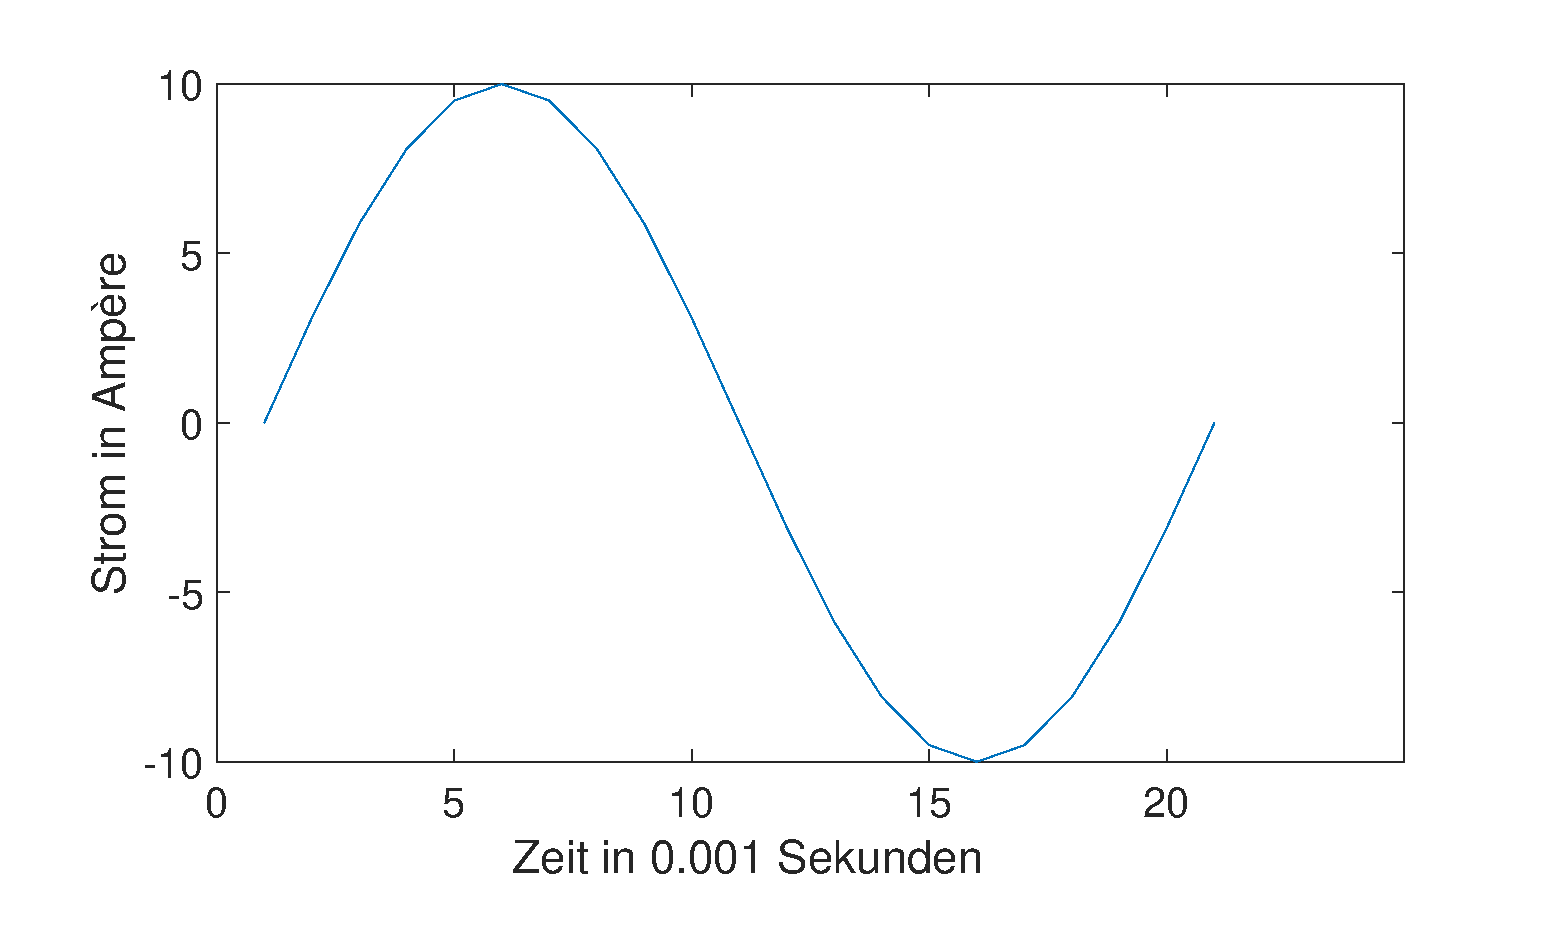
\includegraphics[width=\textwidth]{data/Strom}
	\caption{Anregungsstrom $i(t) = 10\sin(2\pi ft)$}
	\label{fig:Strom}
\end{figure}

Im Postprocessing wird ein Linienplot der Anregung erstellt(siehe Abbildung \ref{fig:Strom}). Außerdem wird für jeden Zeitschritt eine VTK-Datei erstellt zur weiteren Visualisierung des entstehenden Magnetfelds in Paraview.

	\section{Nichtlineare Permeabilität}
Im vorherigen Abschnitt wurde beschrieben, wie man die magnetische Flussdichte innerhalb eines Transformators mit linearem Material simulieren kann. Nun soll im folgenden der gleiche Prozess durchgeführt werden, dieses mal mit einer nicht linearen Kennlinie der Permeabilität. Die Permeabilität hängt hierbei von der magnetischen Flussdichte $B$ ab, da diese zu Beginn der Berechnung nicht bekannt ist muss ein iteratives Verfahren verwendet werden. Die Kennlinie wird durch 
\begin{equation}
	\nu(B) = k_1^{k_2|B|^2} + k_3 \textrm{  mit  } |B| = \sqrt{B^2_x+B^2_y+B^2_z}
\end{equation} beschrieben, wobei $k_1 = 0,3374$, $k_2 = 2,970$ und $k_3 = 388.33$ gilt.\\ \\
Um das entstehende Gleichungssystem der Form \b{A}(\b{x})\b{x} = \b{b} zu lösen wird die Fixpunkt-Iteration verwendet. Man nimmt den Ansatz 
\begin{equation}
	\mb{A}(\mb{x}^{(i)})\mb{x}^{(i+1)}=\mb{b},
\end{equation} wobei die $\mb{x}^{i}$ die Lösung im Schritt $i$ und $\mb{x}^{i+1}$ die Lösung im Schritt $i+1$ beschreibt. Die neue Lösung wird unter Zuhilfenahme der alten Lösung berechnet. Dieses Verfahren ist in dem Skript \tt{trafo\_nichtlinear}, welches im Anhang zu finden ist, mit Hilfe einer while-Schleife implementiert. Die Iteration bricht ab, sobald 
\begin{equation}
	\frac{||\mb{x}^{(i+1)}-\mb{x}^{(i)}||}{||\mb{x}^{(i+1)}||} < 10^{-6}
	\label{eq:norm}
\end{equation} erfüllt ist. Zunächst wird $\mb{x} = \mb{0}$ gewählt, um sicherzustellen, die erste Bedingung der Schleife \tt{i < 2} garantiert, dass mindestens ein \glqq altes\grqq{} und ein \glqq neues\grqq{} berechnet werden. $\mb{A}$ ist in dem zu untersuchenden magnetostatischen Problem durch $\mb{K} = \mb{C}'\mb{M}_\nu \mb{C}$ gegeben. Die linke Seite \b{b} des Gleichungssystems ist der Anregungsstromvektor \b{j}. Die Unbekannte \b{x} stellt das zu berechnende magnetische Vektorpotenzial \b{a} dar. Zusätzlich dazu sind Randbedingungen festgelegt. \\
Bei sehr kleinem Anregungsstrom lässt sich kein magnetisches Feld berechnen, je größer der Anregungsstrom wird, desto mehr Iterationsschritte werden benötigt und dementsprechend dauert die Berechnung länger. Exemplarisch ist das magnetische Feld innerhalb eines Transformators mit einem Anregungsstrom der Spulen von \SI{10}{\ampere} in der Abbildung \ref{fig:BFeld} zu sehen.
\begin{figure}
	\includegraphics[width=\textwidth]{data/BFeld}
	\caption{Das im Transformator entstehende Magnetfeld mit einem Anregungsstrom von \SI{10}{\ampere}}
	\label{fig:BFeld}
\end{figure}
	%%%%%%%%%%%%%%%%%%Fazit%%%%%%%%%%%%%%%%%%%%%%
	%\chapter{Fazit}\label{sec:fazit}
%\addcontentsline{toc}{section}{Fazit}
Die erste Aufgabe ergab, dass sich die beiden Leiter des Koaxialkabels wie die Platten eines Plattenkondensators verhalten. Darüber hinaus ergibt sich, dass man durch Anfügen von weiteren Segmenten an die Schaltung eine Verkleinerung der Schwingfrequenz bewirkt.
Differentialgleichungen können häufig, wie sich in Aufgabe zwei zeigt, leichter im Frequenzbereich als im Zeitbereich gelöst werden. Die durch Lösen der Differentialgleichung analytisch berechneten Ergebnisse für Zeit- und Frequenzverhalten stimmen dabei mit der numerischen Simulation durch LTSpice überein.
Die Ergebnisse der dritten Aufgabe ergeben, dass sich die Feldlinien eines Kondensators in einem Simulationskäfig nicht nur senkrecht zu den Platten bewegen, sondern dass sich auch Randeffekte an den Enden der Kondensatorplatten ausbilden. Untersucht man unterschiedliche Randbedingungen zeigt sich, dass diese sowohl den Kapazitätswert des Kondensators, als auch die elektrischen Feldlinien beeinträchtigen. Die Wahl der Simulationsrandbedingungen kann also nicht willkürlich erfolgen.
	%%%%%%%%%%%%%%%%%%Anhang%%%%%%%%%%%%%%%%%%%%%
	\chapter{Anhang}\label{sec:anhang}
\lstset{ % Octave Settings
	language=Octave,
	extendedchars=true,
	basicstyle=\footnotesize,
	numbers=left,
	numberstyle=\tiny\color{gray},
	stepnumber=1,
	numbersep=10pt,
	showspaces=false,
	showstringspaces=false,
	tabsize=2,
	breaklines=true,
	frame=single,
	morecomment = [l][\itshape\color{blue}]{\%},
	captionpos=b,
	title=\lstname
}


\lstinputlisting{data/SIS.m}
\lstinputlisting{data/SkriptAg8_2.m}
\lstinputlisting{data/SkriptAg8_3d.m}



	%%%%%%%%%%%%%%%%%%%%%%%%%%%%%%%%%%%%%%%%%%%%%%%%%%%%%%%%%%%%%%%%%%%%%%%%%%%%%%%%%%%%%%%%%%%%%%%%%%
	
	%%%%%%%%%%%%%%%%%%%
	%Abbildungs- und Tabellenverzeichnis
	%%%%%%%%%%%%%%%%%%%
	\listoffigures % Abbildungsverzeichnis (captions in den Figuren werden als Referenz genommen)
	%\listoftables % Verzeichnis der Tabellen (captions in den Tabellen werden als Referenz genommen)
	
	%%%%%%%%%%%%%%%%%%%
	%Literaturverzeichnis an dieser Stelle
	%%%%%%%%%%%%%%%%%%%
	
	
\end{document}
